\chapter{Manual de Usuario}
\title{Manual de Usuario}
\label{cap:ManualDeUsuario}

A continuación se detalla un pequeño manual de usuario para aquellos astrónomos ya sean  \textit{amateurs} o profesionales. También se establece para aquellas personas que tengan la curiosidad de descubrir el mundo de la astronomía a través de este prototipo de cliente Web basado en INDI.

\section{Previo}
Antes de comenzar diremos, que si se va a iniciar el prototipo desde un ordenador y se desea lanzar un simulador hay que realizar los siguientes pasos:
\begin{itemize}
  \item Instalar INDI. Para ello hay que instalar INDI en la máquina como dicen los pasos del propio tutorial de la página \cite{InstalarINDI}.
  \item Lanzar Simulador INDI (Figura \ref{fig:INDIServer}). Para lanzar un simulador INDI hay que abrir un terminal en Linux \cite{Linux} y escribir la siguiente instrucción si se desea lanzar por ejemplo un telescopio:\\
  \texttt{> indiserver indi\_simulator\_telescope}
\end{itemize}

Al presionar la tecla Enter, hemos lanzado nuestro simulador de telescopio, en este caso. Si se desea lanzar otro simulador tiene que proceder de la misma manera, o sea, repetir la operación de la forma “Lanzar Simulador INDI” y cambiar el nombre del dispositivo por el que se desea ejecutar. Por ejemplo:\\
\texttt{> indiserver indi\_simulator\_ccd}\\
\texttt{> indiserver indi\_simulator\_gps}\\

La lista de dispositivos se puede consultar en la dirección que a continuación se facilita \cite{ListaDispositivos}.

\begin{figure}[htb]
\centering
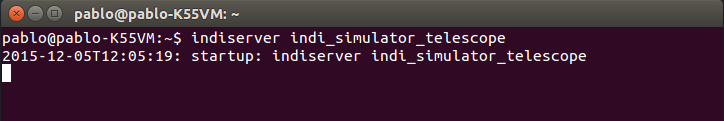
\includegraphics[width=1\textwidth]{./imagenes/capturaINDIServer}
\caption{Lanzamiento del Simulador de Telescopio} \label{fig:INDIServer}
\end{figure}

\section{Lanzando el Prototipo de Cliente}
Una vez que está lanzado el simulador con el que vamos a trabajar, tenemos que abrir el fichero principal denominado \textit{parser.html}.

En el momento que tengamos abierto el fichero \textit{parser.html} en el navegador, se nos solicitará una IP y un puerto válido que corresponderá con un servidor INDI (Figura \ref{fig:conexionINDI}).\\

Al conectar con el servidor, nos aparecerá una ventana correspondiente al dispositivo que estamos simulando. Por el contrario, si no se ha lanzado ningún simulador, al conectar con el servidor se mostrarán los diferentes dispositivos conectados con el servidor en ese momento. \\

Cada dispositivo se muestra en una ventana y a partir de ahí se puede interaccionar con él realizando todas las modificaciones que se quieran, analizando los datos que se obtienen, etc.
\begin{figure}[htb]
\centering
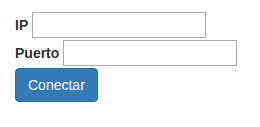
\includegraphics[width=0.7\textwidth]{./imagenes/capturaConexion}
\caption{Conexión con el Servidor INDI} \label{fig:conexionINDI}
\end{figure}

\section{Encender un Dispositivo}
Cuando se ha realizado la conexión con el servidor y hemos lanzado algún simulador hay que tener en cuenta que, por regla general, el dispositivo estará apagado. Su pantalla principal tendrá un desplegable para realizar la función de conexión. Además de ese desplegable, es posible que tenga una pestaña que pertenezca a un grupo, que será el de Opciones, con el nombre del dispositivo, su versión y algunos datos referentes al dispositivo. \\

Una vez que en la pestaña principal del dispositivo se inicia la conexión, se muestran todos los grupos de Propiedades y sus correspondientes y específicas propiedades para interactuar con el dispositivo.
\begin{figure}[htb]
\centering
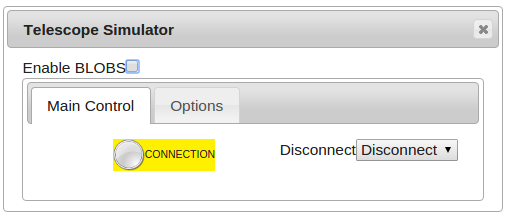
\includegraphics[width=0.9\textwidth]{./imagenes/capturaEncendiendo}
\caption{Encendiendo un Dispositivo} \label{fig:encendiendoDispositivo}
\end{figure}

\section{Interactuar con un Dispositivo}
Cuando se establece la conexión y encendemos el dispositivo, tenemos acceso a toda su información  que está agrupada en diferentes grupos podemos decir que ya estamos conectados con el dispositivo (Figura \ref{fig:capturaDispositivo}).\\

Hay que tener bien claro que las propiedades se pueden o no modificar, dependiendo del tipo de permiso que tengan. Las propiedades que se pueden modificar tendrán un desplegable, un cuadro de texto, un cuadro numérico o un \textit{checkbox}. Además hay que decir, que salvo los desplegables, las demás propiedades tendrán siempre un botón para poder actualizar los diferentes valores y enviarlos así al servidor.
\begin{figure}[htb]
\centering
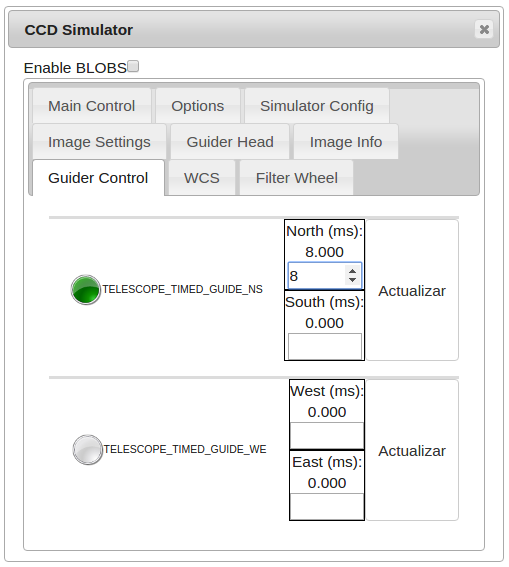
\includegraphics[width=0.8\textwidth]{./imagenes/capturaDispositivo}
\caption{Dispositivo CCD Encendido} \label{fig:capturaDispositivo}
\end{figure}

\subsection{Estado de una Propiedad}
Cada propiedad tiene un estado asociado a ella que se muestra en forma de luz y que corresponde con las siguientes luces:
\begin{itemize}
  \item 
\includegraphics[width=0.5cm]{./imagenes/grey_light} \textbf{Inactivo:} La propiedad está sin establecer.
  \item 
\includegraphics[width=0.5cm]{./imagenes/yellow_light} \textbf{Ocupado:} La propiedad está ajustando algún valor.
  \item 
\includegraphics[width=0.5cm]{./imagenes/red_light} \textbf{Alerta:} Hay algún problema con la propiedad.
  \item 
\includegraphics[width=0.5cm]{./imagenes/green_light} \textbf{Ok:} Todos los valores de la propiedad son correctos.
\end{itemize}

\subsection{Cambio de Grupo de Propiedades}
Para cambiar del grupo de propiedades basta con pulsar en las diferentes pestañas que tiene el dispositivo. Las pestañas sirven para agrupar propiedades. Dentro de la misma pestaña se encuentran acogidas todas aquellas propiedades que corresponden al mismo tipo, formando un conjunto específico de propiedades en una única y diferente pestaña. De este modo, cada grupo de propiedades del mismo tipo se encontrarán en su correspondiente pestaña (Figura \ref{fig:gruposPropiedades}).
\begin{figure}[htb]
\centering
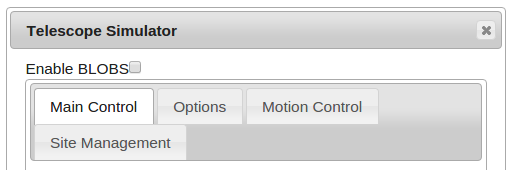
\includegraphics[width=1\textwidth]{./imagenes/capturaGrupos}
\caption{Grupos de Propiedades del Telescopio} \label{fig:gruposPropiedades}
\end{figure}

\subsection{Cambio de una Propiedad \textit{Text}}
Las propiedades \textit{text} son aquellas que sirven para dar nombre a las diferentes partes del dispositivo.
La propiedad se puede modificar utilizando caracteres alfanuméricos y seguidamente pulsando el botón actualizar. Realizada esta operación, la propiedad queda modificada (Figura \ref{fig:propiedadText}).
\begin{figure}[htb]
\centering
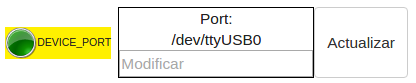
\includegraphics[width=0.8\textwidth]{./imagenes/capturaText}
\caption{Propiedad \textit{Text} del Telescopio} \label{fig:propiedadText}
\end{figure}

\subsection{Cambio de una Propiedad \textit{Number}}
Las propiedades \textit{number} son aquellas que muestran unicamente números. Tienen la particularidad de que solamente se pueden cambiar por parámetros que sean numéricos. Cada propiedad \textit{number} tiene un formato que se especifica al pasar el cursor por encima del cuadro numérico. Si se introduce un valor que está fuera del rango o no está en el formato que se solicita, aunque se pulse el botón actualizar el valor no cambiará (Figura \ref{fig:propiedadNumber}).
\begin{figure}[htb]
\centering
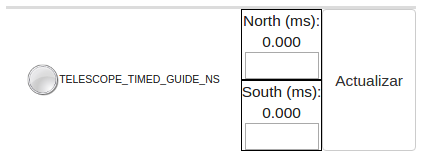
\includegraphics[width=1\textwidth]{./imagenes/capturaNumber}
\caption{Propiedad \textit{Number} del Telescopio} \label{fig:propiedadNumber}
\end{figure}

\subsection{Cambio de una Propiedad \textit{Switch}}
Se agrupan en tres grupos según del tipo al que pertenezca:
\begin{itemize}
  \item \textbf{\textit{One Of Many}:} Siempre estará un valor seleccionado y se puede modificar con cualquier valor del desplegable (Figura \ref{fig:oneOfMany}).
  \begin{figure}[htb]
  \centering
  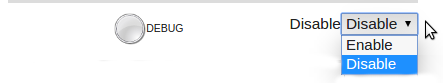
\includegraphics[width=0.8\textwidth]{./imagenes/oneOfMany}
  \caption{Propiedad \textit{Switch - One Of Many} del Telescopio} \label{fig:oneOfMany}
  \end{figure}
  \item \textbf{\textit{At Most One}:} Se puede seleccionar uno o ninguno de los valores que hay en el desplegables (Figura \ref{fig:atMostOne}).
  \begin{figure}[htb]
  \centering
  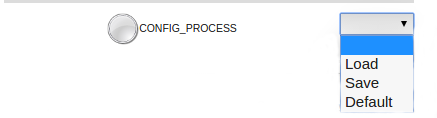
\includegraphics[width=0.8\textwidth]{./imagenes/atMostOne}
  \caption{Propiedad \textit{Switch - At Most One} del Telescopio} \label{fig:atMostOne}
  \end{figure}
  \item \textbf{\textit{Any Of Many}:} Se pueden seleccionar todos los valores que se deseen de los diferentes \textit{checkbox} que aparecen (Figura \ref{fig:anyOfMany}).
  \begin{figure}[htb]
  \centering
  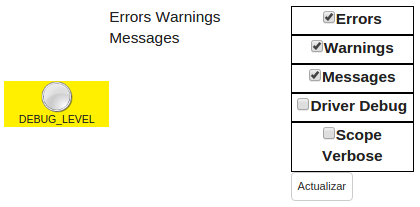
\includegraphics[width=0.9\textwidth]{./imagenes/anyOfMany}
  \caption{Propiedad \textit{Switch - Any Of Many} del Telescopio} \label{fig:anyOfMany}
  \end{figure}
\end{itemize}

Hay que resaltar que tanto en los desplegables como en los \textit{checkbox}, el nombre o nombres seleccionados y que se han enviado al servidor aparece a la izquierda de los propios desplegables o \textit{checkbox}.

\subsection{Activar/Desactivar la Recepción de \textit{Blob}}
Cada dispositivo establece la posibilidad de habilitar la recepción de \textit{blob} que por defecto, viene desactivada para todos los dispositivos. Para activarla tan solo hay que marcar la casilla de \textit{Enable BLOBS} que se encuentra en la parte superior de la ventana del dispositivo (Figura \ref{fig:activacionBlob}).
\begin{figure}[htb]
\centering
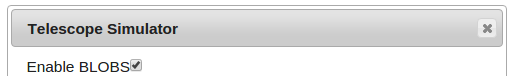
\includegraphics[width=0.9\textwidth]{./imagenes/activacionBlob}
\caption{Activación de Recepción de \textit{Blob} del Telescopio} \label{fig:activacionBlob}
\end{figure}

\subsection{Cerrar un Dispositivo}
Para ello, tan solo hay que darle a la X de la ventana y se cierra ese dispositivo. Hay que destacar que no se finaliza la conexión con él porque haciendo esa operación, lo único que se produce es el cierre de la ventana pero no de la conexión. Hasta que no se cierra la ventana del navegador, el dispositivo sigue conectado.
